\subsection{Section 6.1 Triangulating Spaces}
\label{sec:Triangulating-Spaces}

He gave to examples first,
\begin{ex}
    A trivial example:
    \begin{figure}[H]
        \centering
        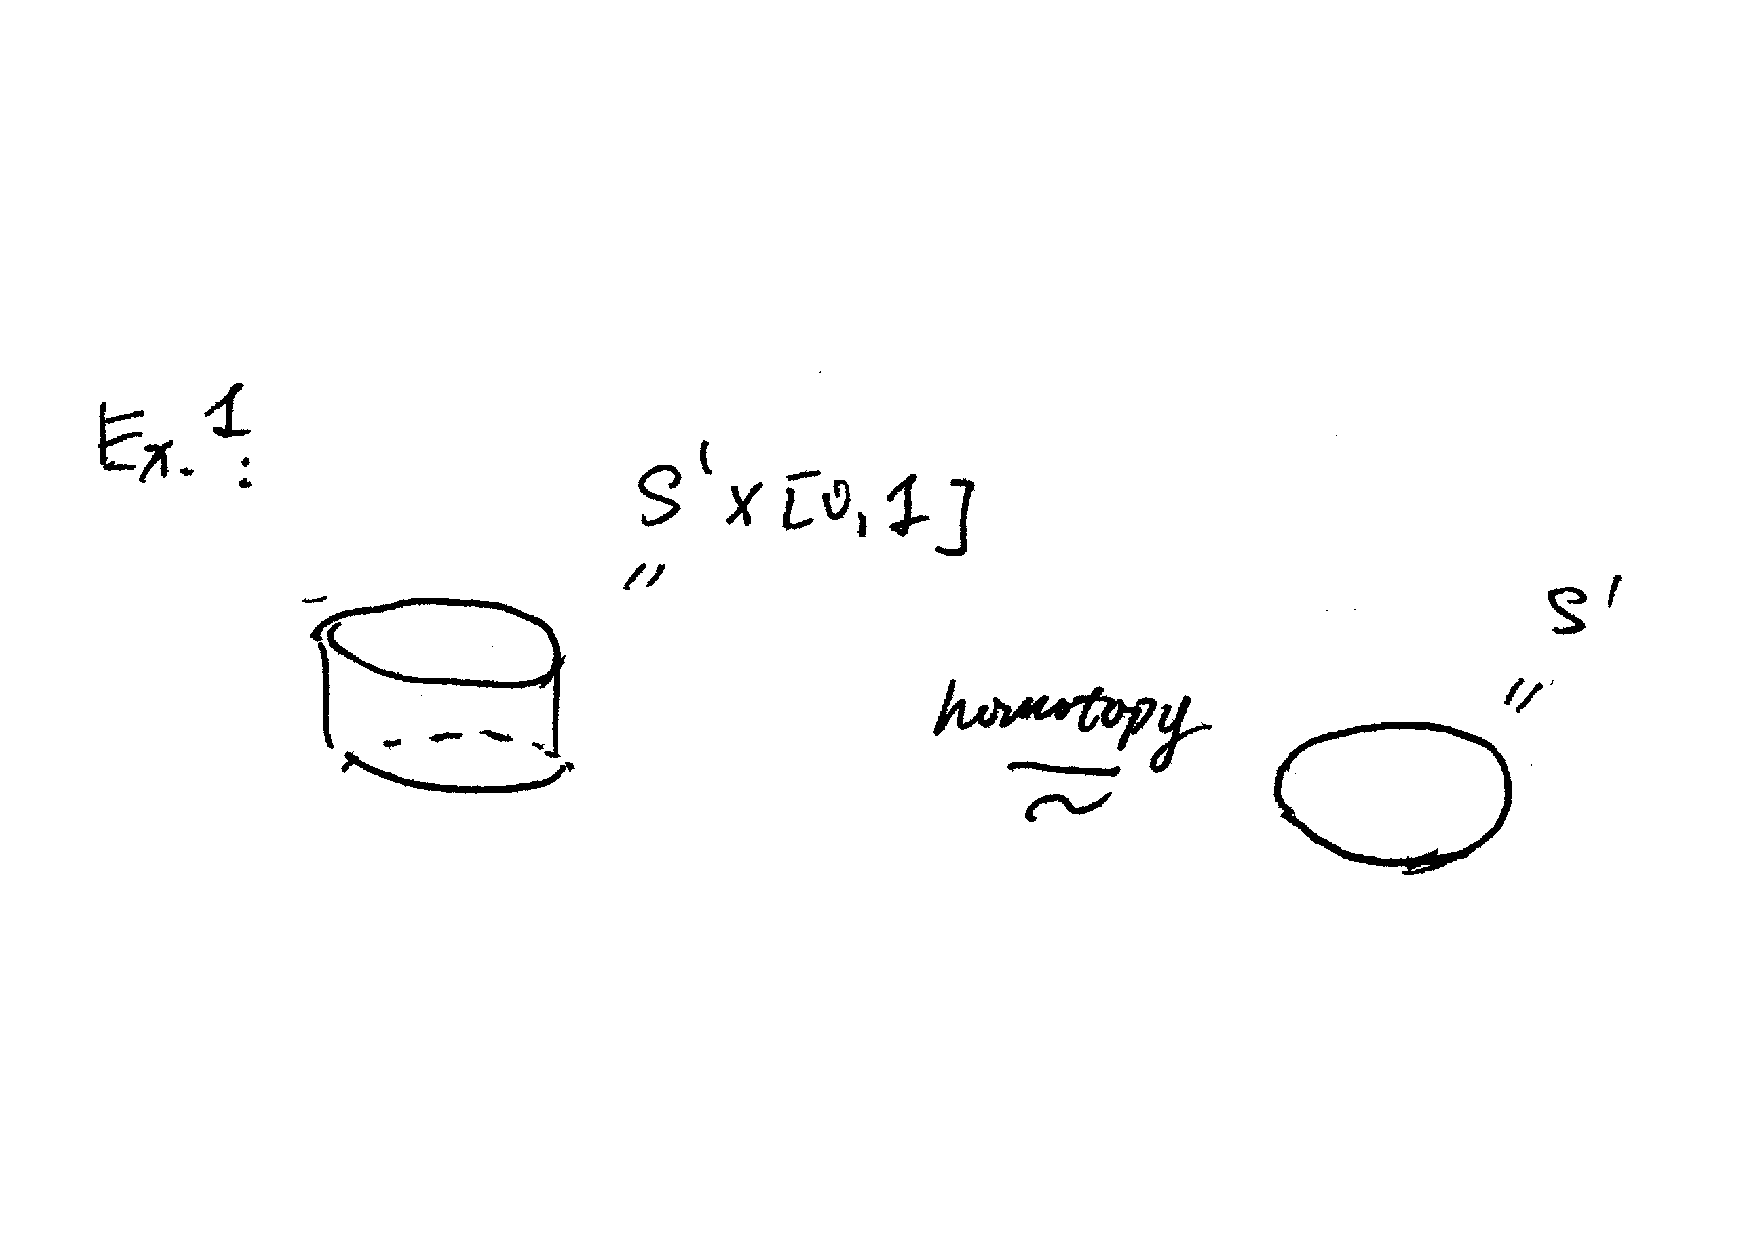
\includegraphics[width=0.6\linewidth]{pics/ch6-scanned-notes-1/ex1.pdf}
    \end{figure}
\end{ex}
\begin{ex}
    A non trivial one. That is, the M\"obius Strip also has the
    homotopy type of a ciclr $S^1$.
    \begin{figure}[H]
        \centering
        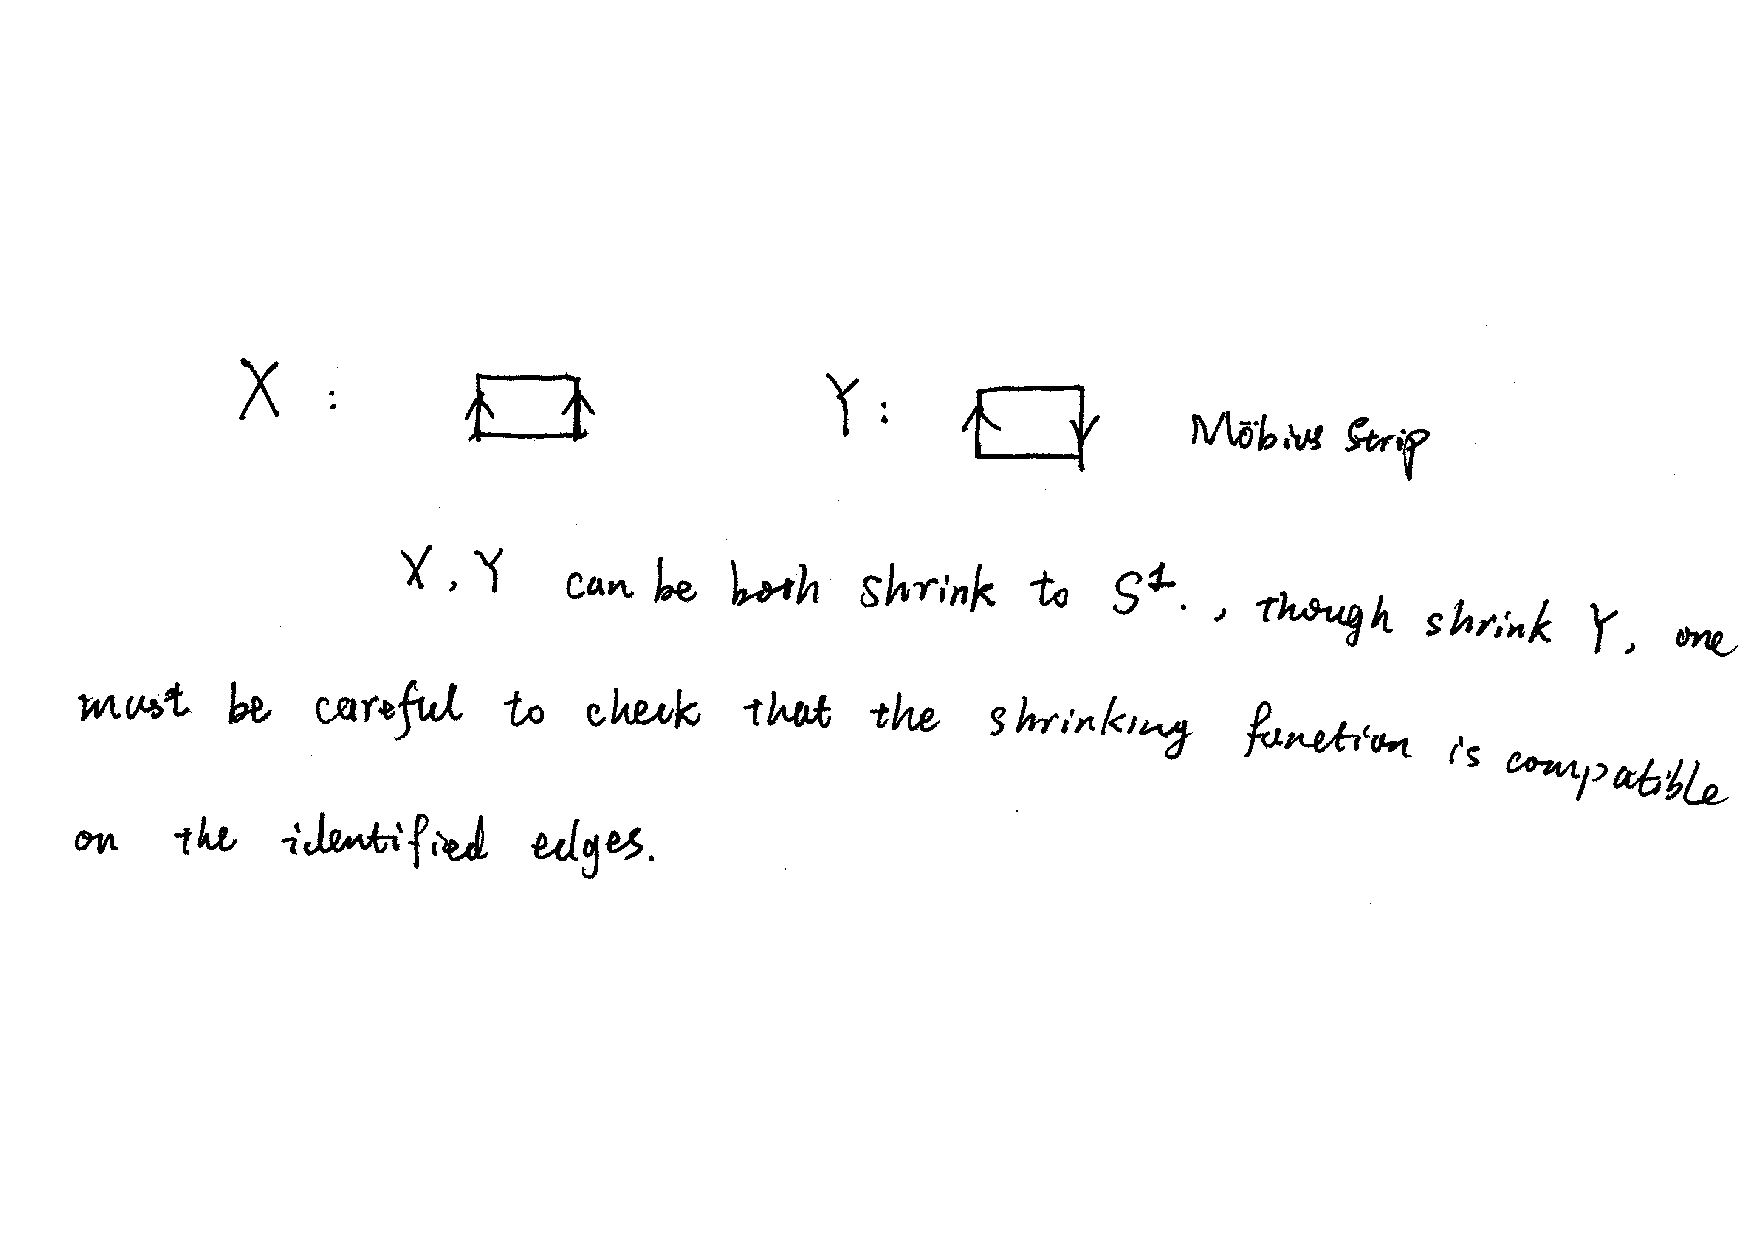
\includegraphics[width=0.8\linewidth]{pics/ch6-scanned-notes-1/ex2.pdf}
    \end{figure}
\end{ex}
But for complicated spaces, its homotopy type will not be so easy to
calculate in with simple imagination. Here we will introduce a new
technique to actually calculate the homotopy type of topological
spaces.

The technique is called Triangulation. The most visual example comes
from the computer vision technology (though I cannot find a picture by
directly Googling triangulation). The idea we wants to stress is that
the Triangulation is like use small patches of triangles to patch and
cover the surface of 3D smooth objects. Increase the overall number of
patches and make each patch get smaller. In the limit of this process
one might get to recover the original image.

\begin{defi}[Simplex of $\dim k$]
\nomenclature{Simplex of $\dim k$}{\nomrefpage.}
    The stanford simplex of $\dim k$ in $R^{k+1}$ is defined as
    follows. Let $v_i=(0,\cdots,0,1,0,\cdots 0)$, where $1$ is in $i+1$
    coordinates. That is:
    $$ v_0=(1,0,\cdots)$$
    $$ v_1=(0,1,0\cdots)$$
    $$\cdots$$
    $$ v_0=(0,\cdots,0,1)$$
    Then the simplex is the smallest convex set containing
    $\{v_0,\cdots,v_k\}$ in $\R^{k+1}$. It is also called a
    \nomen{$k$-simplex}.
\end{defi}
\begin{ex}
    \begin{figure}[H]
        \centering
        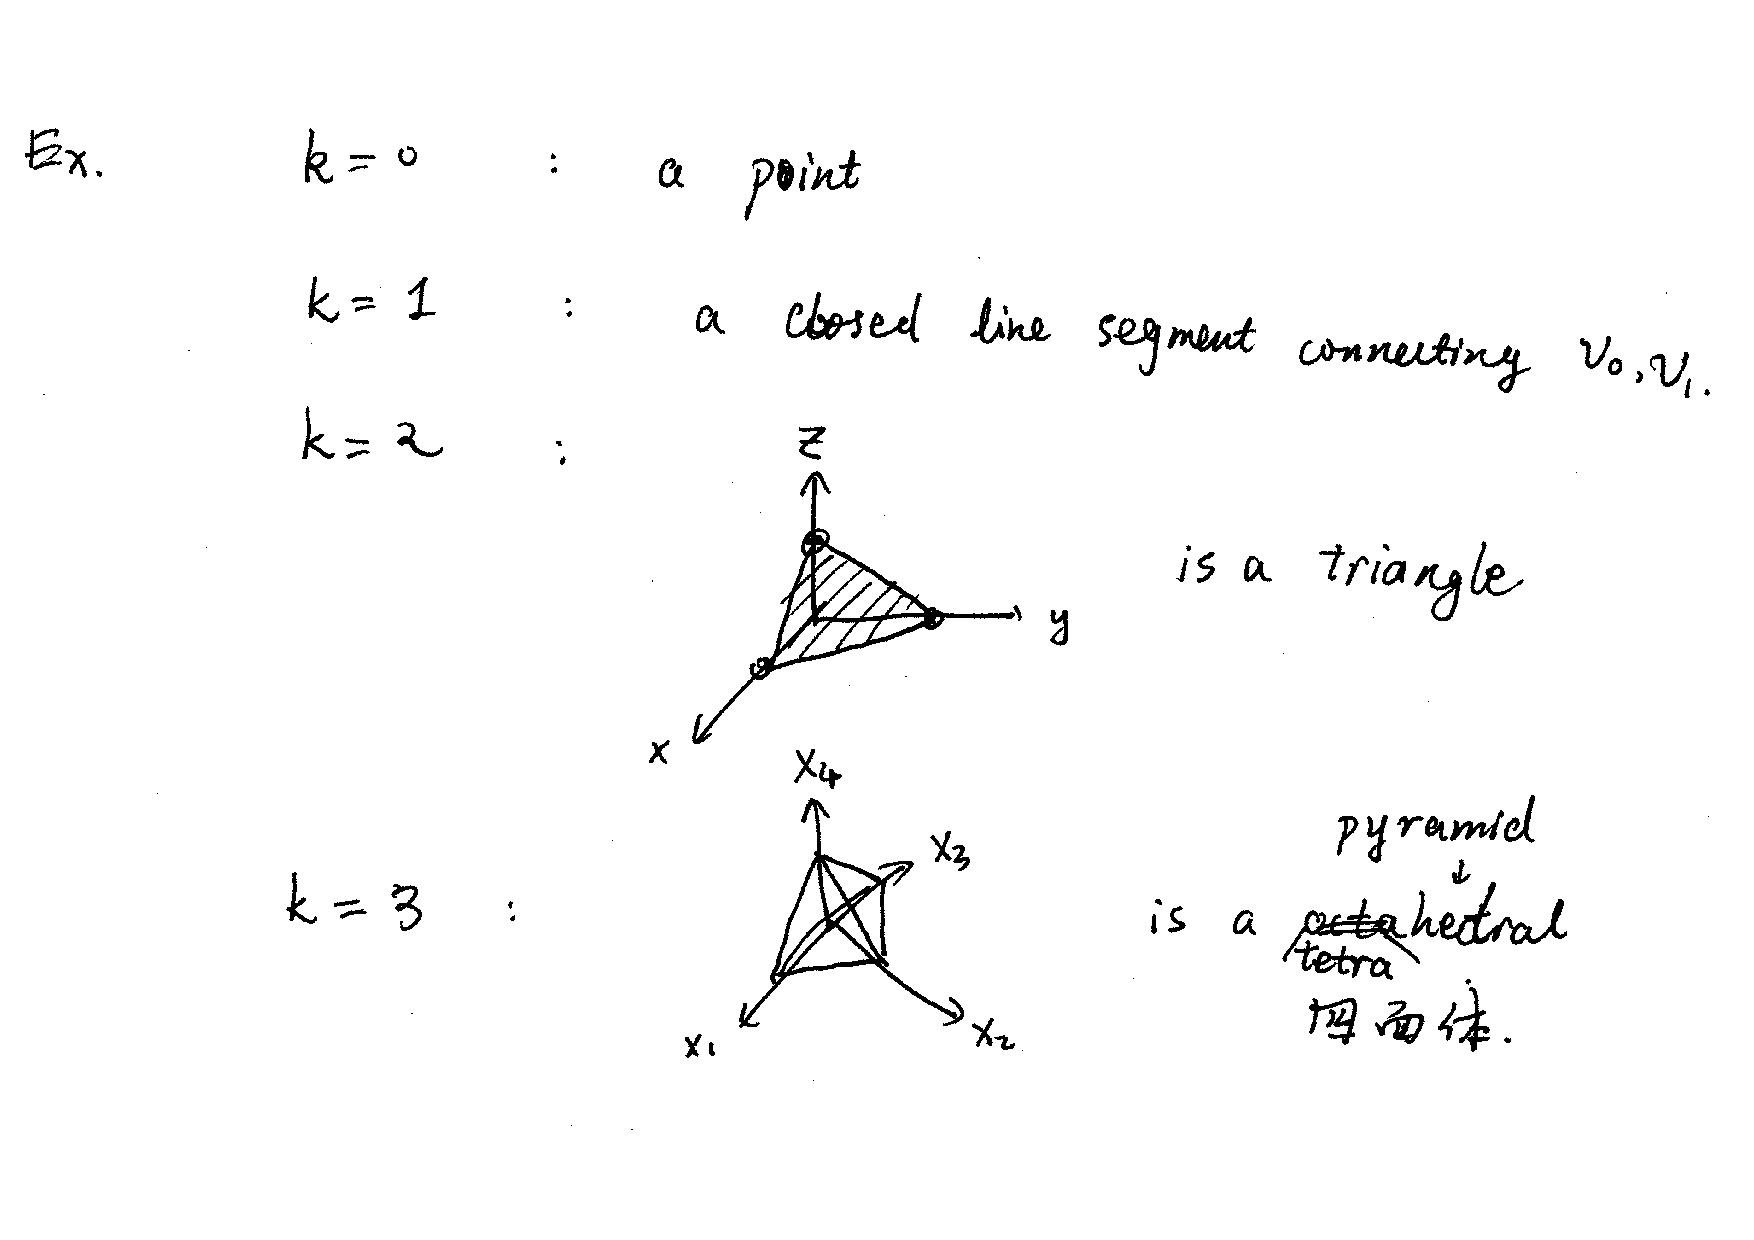
\includegraphics[width=0.8\linewidth]{pics/ch6-scanned-notes-1/ex3.pdf}
    \end{figure}
\end{ex}
\begin{fact}
    Any point in a $k$-simplex is of the form:
    \begin{equation}
        \lambda_0 v_0 + \lambda_1 v_1 + \cdots + \lambda_k v_k
    \end{equation}
    where each $\lambda_i\geq 0$, and $\sum_{i=0}^{k} \lambda_k=1$.
\end{fact}
\begin{ex}
    There is a special point in the $k$-simplex:
    \begin{equation}
        \frac{1}{k+1} \sum_{i=0}^k v_i
    \end{equation}
    When $k=2$, this is just the usual center of gravity of triangle.
\end{ex}

We want to study those space which is the union of a finite collection
of simplexes which fit together nicely in some Euclidean space. These
are called "triangulable spaces". More specifically:
\begin{defi}[faces]
\nomenclature{faces}{\nomrefpage.}
    If $A$ and $B$ are simplexes, and if the vertices of $B$ form a
    subset of vertices of $A$. Then $B$ is called a face of $A$,
    written as \nomen{$B<A$}.
\end{defi}
\begin{defi}[Simplicial Complex]
\nomenclature{Simplicial Complex}{\nomrefpage.}
    A \textbf{finite} collection of simplexes in some Euclidean space
    in $\R^n$ is called a simplicial complex, if
    \begin{enumerate}
        \item whenever a simplex lies in this collection, then so does
            its faces
        \item whenever two simplexes in this collection intersect,
            their intersection is a common face of these two
            simplexes.
    \end{enumerate}
\end{defi}
\begin{ex}
    % ex 4
\end{ex}
\begin{defi}[Topology on simplicial complex]
\nomenclature{Topology on simplicial complex}{\nomrefpage.}
    The topology on a simplicial complex is given by the subspace
    topology of Euclidean space. Let $K$ be a simplicial complex, we
    denote \nomen{$|K|$} as the topology of $K$. This $|K|$ is called
    a \nomen{polyhedron}.
\end{defi}

\begin{defi}[Triangulation and Triangulable]
\nomenclature{Triangulation and Triangulable}{\nomrefpage.}
    A triangulation on a topological space $X$ consists of a
    simplicial complex $K$, and a homeomorphism $h$:
    $$ h:|K|\to X$$
    A space is called triangulable if such simplicial complex $|K|$
    and homeomorphism $h$ exists.
\end{defi}
\begin{fact}
    If $X$ is triangulable, then $X$ is compact and can be made into a
    metric space. (Notice that the simplicial complex is a finite
    collection.)
\end{fact}
\begin{remark}
    Trigulation is in general not unique. For example:
    \begin{figure}[H]
        \centering
        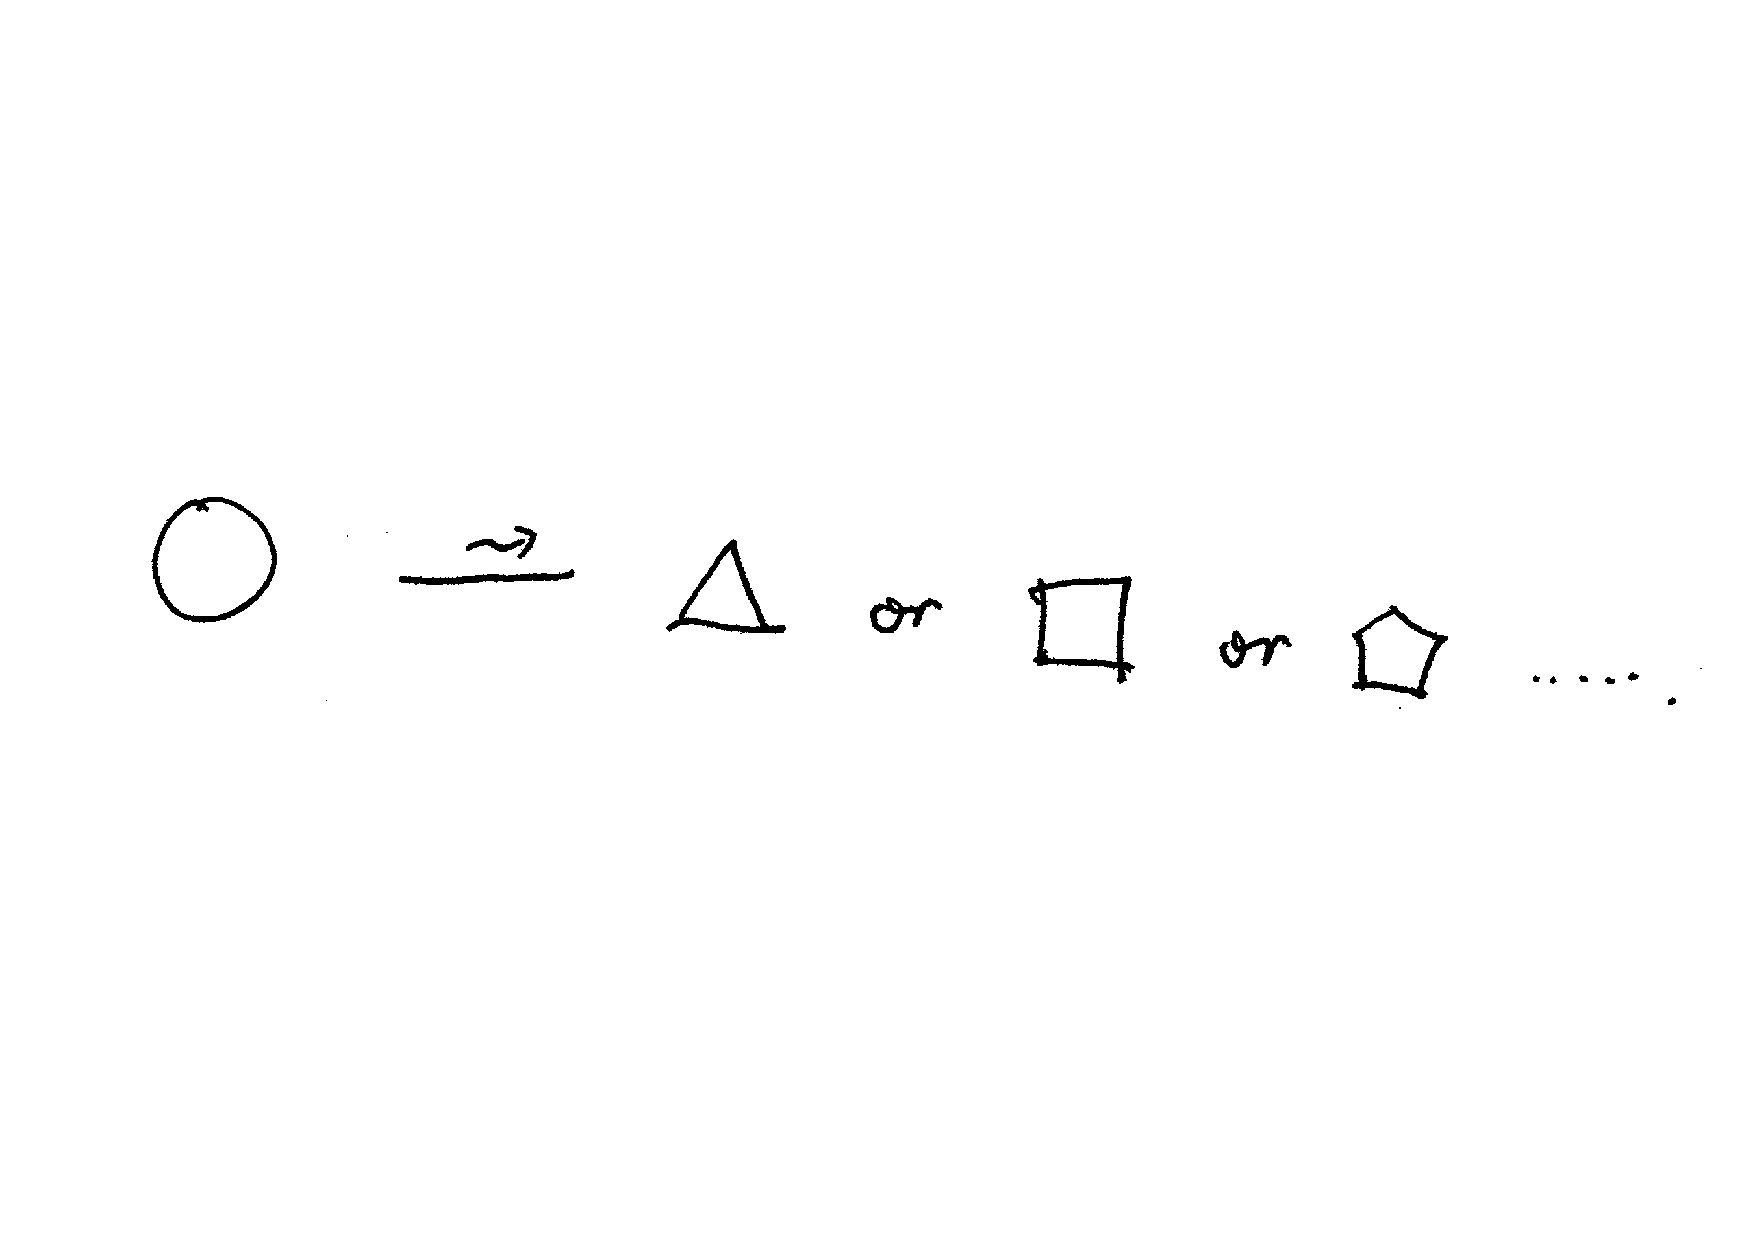
\includegraphics[width=0.6\linewidth]{pics/ch6-scanned-notes-1/rmk2}
    \end{figure}
\end{remark}
\begin{ex}
    Here is a triangulation on the torus:
    \begin{figure}[H]
        \centering
        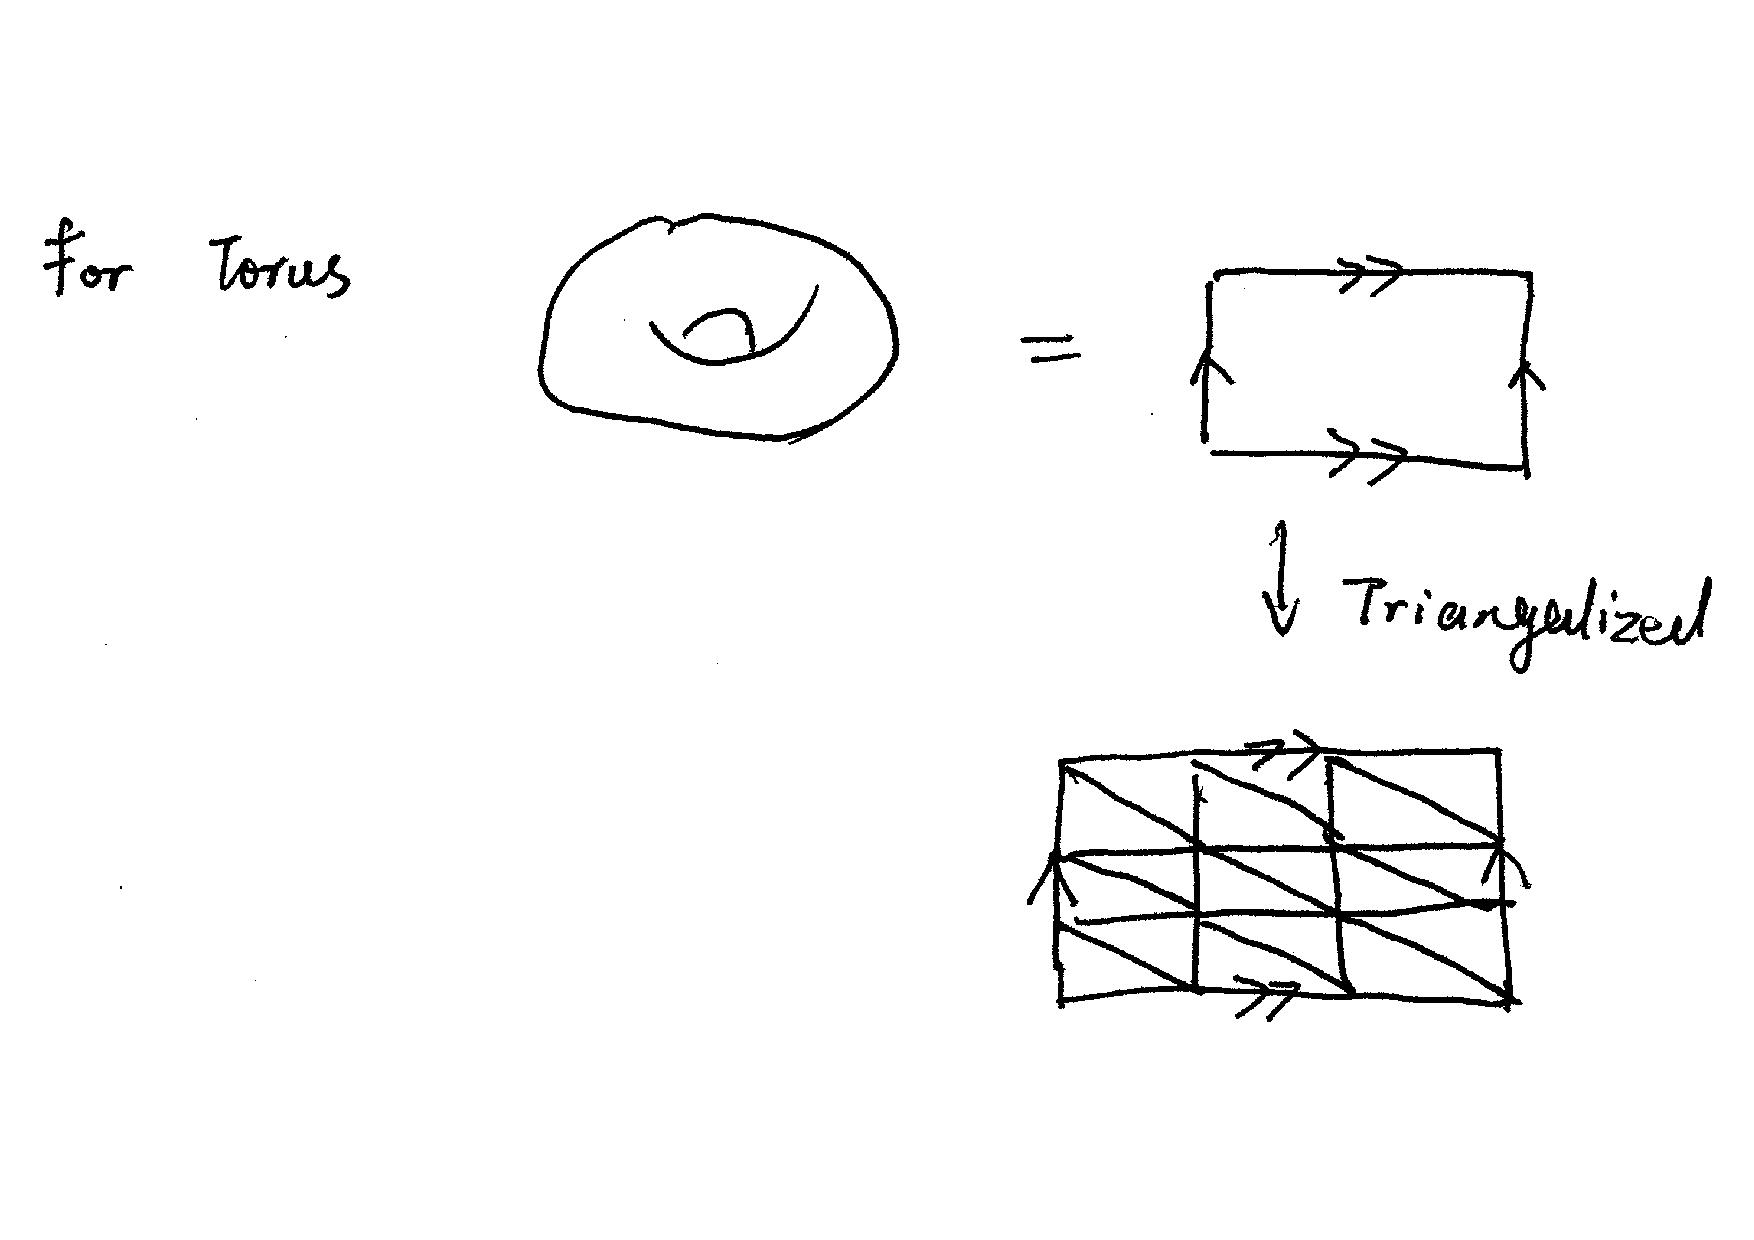
\includegraphics[width=0.6\linewidth]{pics/ch6-scanned-notes-1/p5.pdf}
    \end{figure}
    Notice that the following diagram is not a triangulation of torus:
    \begin{figure}[H]
        \centering
        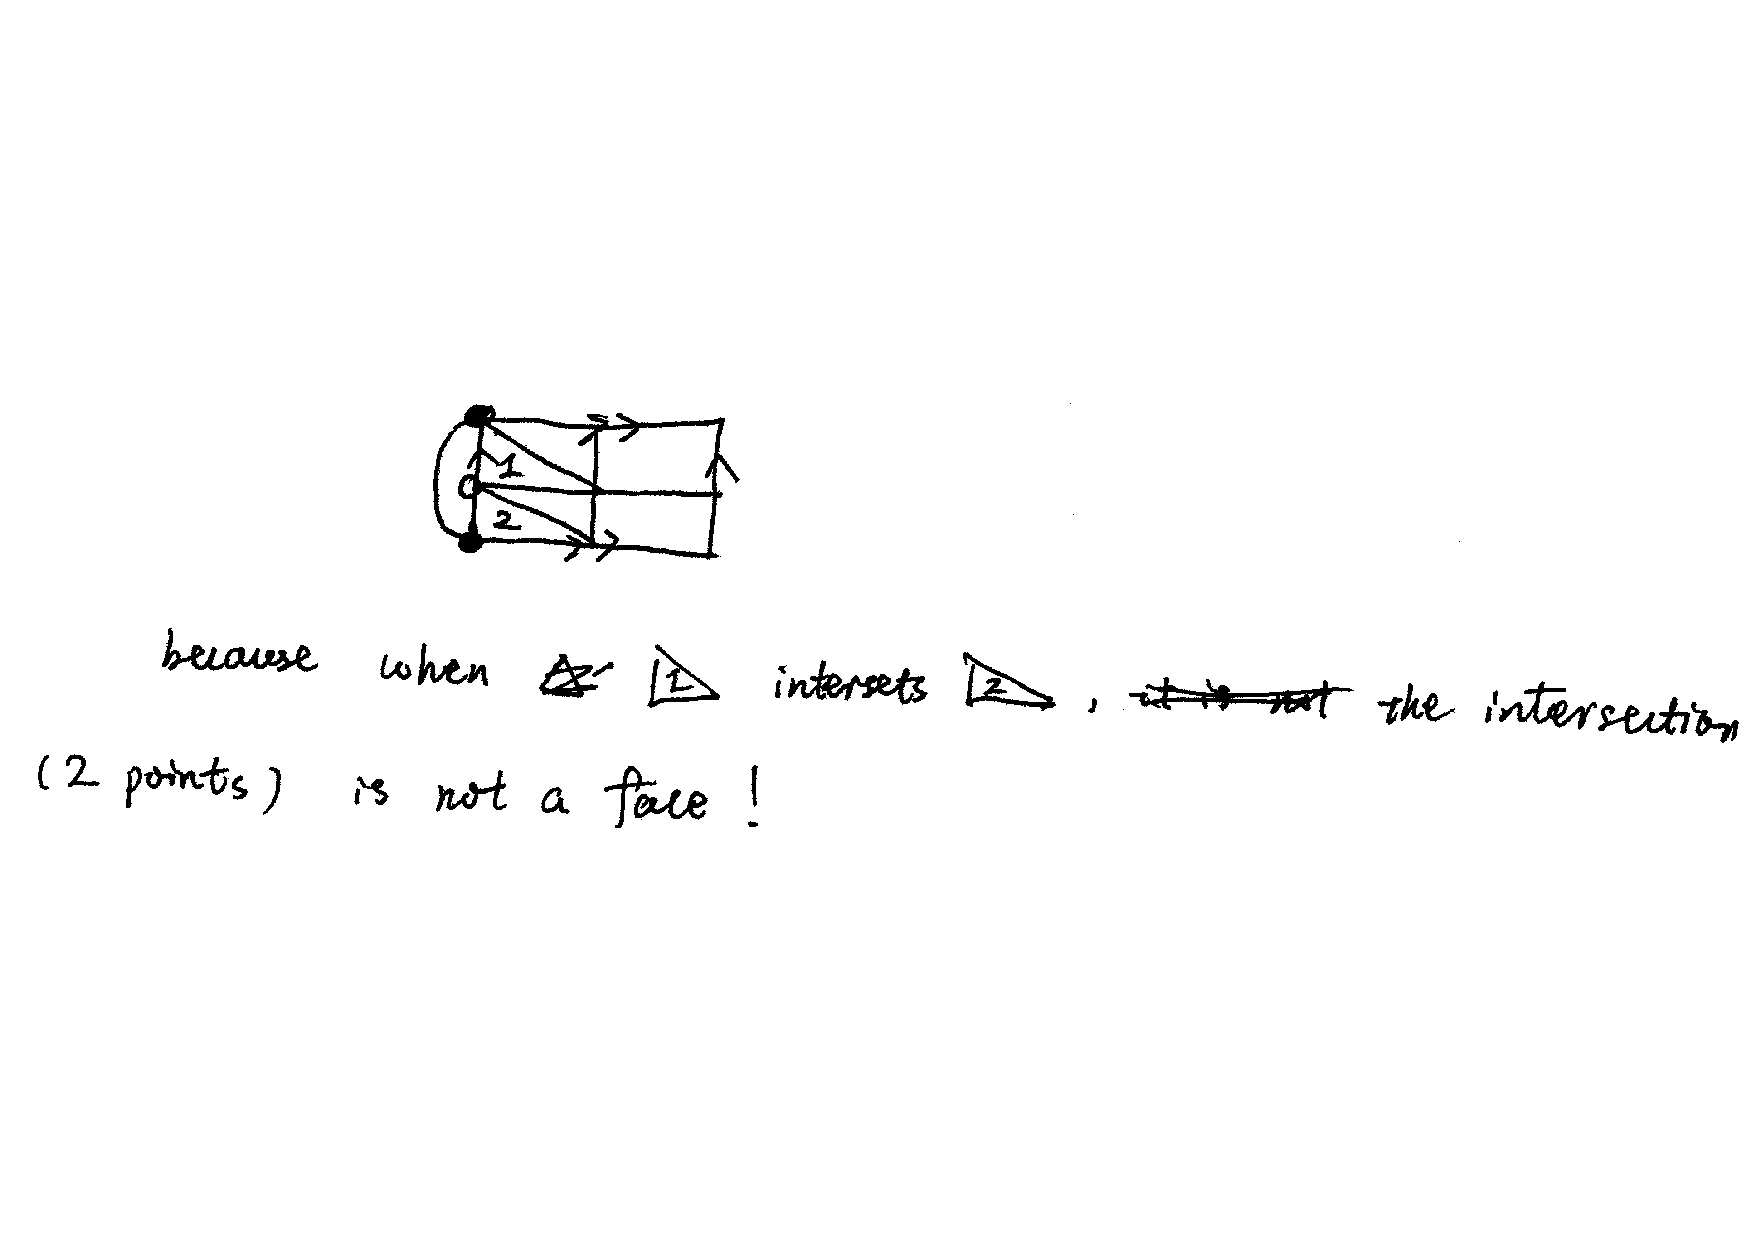
\includegraphics[width=0.8\linewidth]{pics/ch6-scanned-notes-1/p52.pdf}
    \end{figure}
\end{ex}
\begin{lemma}
    Let $K$ be a simplicial complex in $\R^{n}$, then
    \begin{enumerate}
        \item $|K|$ is compact.
        \item Each point of $|K|$ lies in the interior of exactly one
            simplex of $K$.
        \item If we take the simplexes of $K$ seperately, and give
            their union the identification topology, we obtain $|K|$.
            Thus we have two equivalent ways to view the topology on
            $K$.
        \item If $|K|$ is connected, then $|K|$ is also
            path-connected.
    \end{enumerate}
\end{lemma}
\begin{proof}
\begin{enumerate}
    \item Obviously.
    \item Since $K$ is connected by simplexes, a point $p$ must
        obviously be contained in some simplex. Also, since on each
        simplex $p$ must be on the interior of it, or interior of its
        components. We only need to prove that the containing simplex
        is unique. Suppose $p$ is the interior of simplexes $A$ and
        $B$. Notice that their intersection must be their faces. The
        only face of $A$ or $B$ containing interior points is $A$ or
        $B$ itself. Hence $A=B$.
    \item By definition of identification topology, we can see that in
        the identified space, a subset $C\subset |K|$, $C$ is closed
        $\Leftrightarrow$ $C\cap |A|$ is closed in $|A|$ for all
        simplexes $A\in K$. The rest of the proof is obvious.
    \item We need only to show that $|K|$ is locally path-connected.
        But any point $p\in K$, $p\in$ interior of some $A$ where
        $A\in K$. That is, we can find a neighbourhood $U$ of $p$, and
        $U$ is contained in $A$ ($U\subset A$). (More specifically, we
        can find $\varepsilon$ such that 
        $B_{\varepsilon}(p)\cup |K| = B_\varepsilon(p)\cup |A|$)
        But a simplex $A$ is obviously locally path-connected. Hence
        $U$ (or $B_\varepsilon(p)$) is path connected, hence $|K|$ is
        path-connected.
\end{enumerate}
\end{proof}

\subsection{Section 6.2 Barycentric Division}
\label{sec:Barycentric-Division}
Now we begin to make the triangulation more and more detailed. We
start from a simplicial complex $K$ and constructing a new simplicial
complex $K_1$, such that
\begin{enumerate}
    \item $|K|=|K_1|$, homeomorphically.
    \item diameter $|K_1|<$ diameter $|K|$.
\end{enumerate}
The general construction method is called Barycentric division,
visualized as:
\begin{figure}[H]
    \centering
    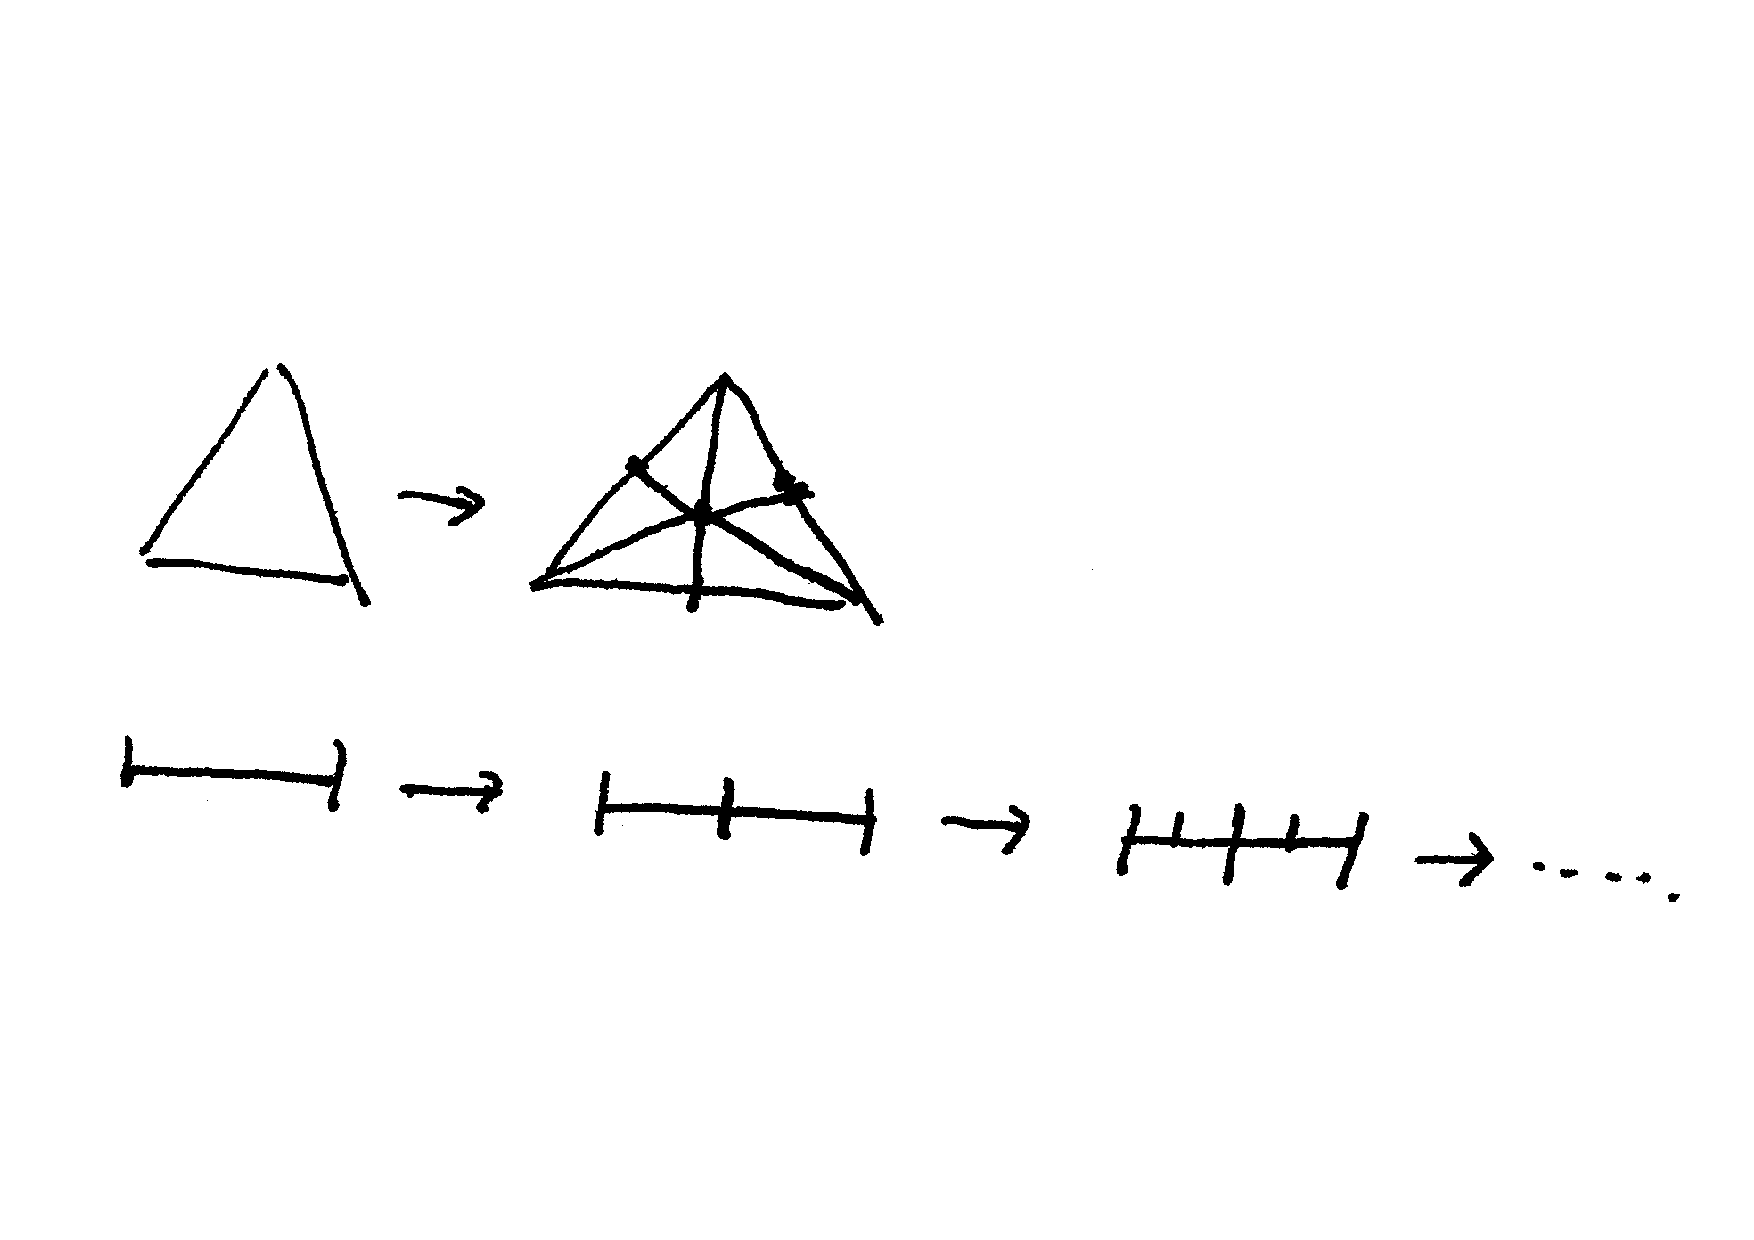
\includegraphics[width=0.6\linewidth]{pics/ch6-scanned-notes-1/8.pdf}
\end{figure}
We first define a concept
\begin{defi}[$\hat{A}$ Bary center]
\nomenclature{$\hat{A}$ Bary center}{\nomrefpage.}
Let $A$ be a simplex, then the bery center of $A$, denoted $\hat{A}$,
is the point:
\begin{equation}
    \hat{A}:= \frac{1}{k+1}(v_0+\cdots+v_k)
\end{equation}
\end{defi}
Then, the general process is:
The new space $K_1$ is such that
\begin{enumerate}
    \item The vertices of $K_1$ are bary centers of \textbf{ALL}
        simplexes of $K$. Note the the bary center of a $0$-simplex
        is just itself. So in general, $K_1$ has more vortices of
        $K$.
    \item A collection $\hat{A}_0,\cdots,\hat{A}_k$ of such bary
        centers will form a vortex of a $k$-simplex in $K_1$ if and
        only if there is a permutation $\sigma$ of $\{0,1,\cdots,k\}$
        such that
        \begin{equation}
            A_{\sigma{0}}< A_{\sigma{1}} < \cdots < A_{\sigma{k}}
        \end{equation}
\end{enumerate}
\begin{remark}
    The second point above tries to do the following
    \begin{figure}[H]
        \centering
        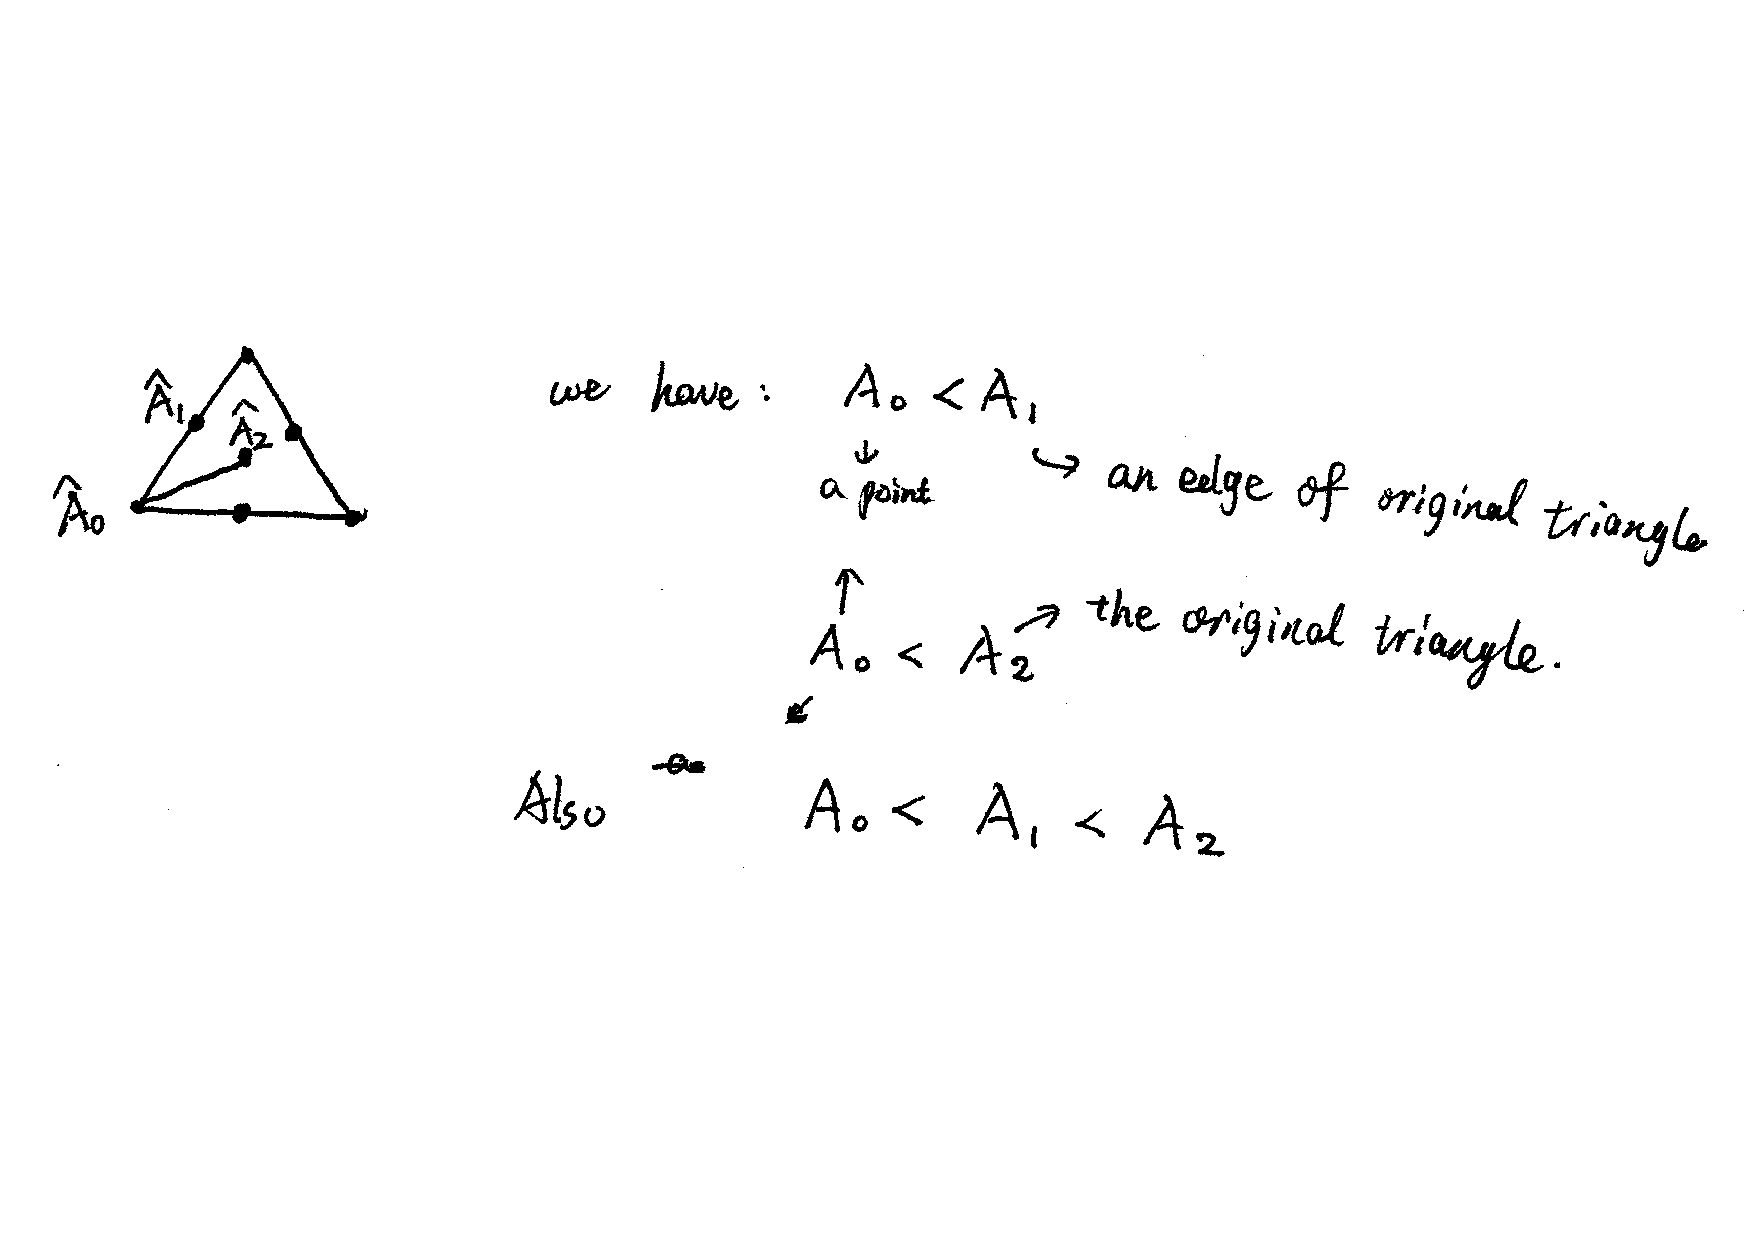
\includegraphics[width=0.9\linewidth]{pics/ch6-scanned-notes-1/p9.pdf}
    \end{figure}
\end{remark}

Now we give a precise de
